\section{Models}
As said in the introduction we first tested the k-neighbors classifier (KNN), multilayer perceptron (MLP), random forest classifier (RFC) and support vector machine (SVM) algorithms individually with the original Morgan fingerprint. We also tried decision tree classifier (DTC) and linear discriminant analysis (LDA) but they were a lot worse than the others.

The estimations gravitated around \SI{74}{\percent}, but when we submitted these algorithms, the results were quite poor ($\sim$\SI{71}{\percent}) in comparison. We then realized that using the \texttt{useFeature = True} parameter significantly increased the score for both our estimations and Kaggle scores. Since we don't know much about organic chemistry, the consequences of this parameter are kind of blurry in our mind. Yet from what we understood, when set to \texttt{True}, the algorithm will detect feature-based invariants (predefined patterns) within the molecule \cite{scikit-morgan-features}.

At the same time, we noticed the parameters \texttt{nBits} (the number of bits in the bit vector) and \texttt{radius}. But, since we didn't want our scripts to run for too long, we didn't increase the number of bits until the end of our parameters testing phase, which was unfortunate as increasing that parameter usually provided better results (but induced computation times that were much longer).

In the following, if it not precised, the fingerprint used is Morgan, the number of bits $128$, the radius $2$ and the parameter \texttt{useFeature} is \texttt{True}.

\subsection{K-Neighbors classifier}

The parameter influencing the score of this method are the number of neighbors considered (\texttt{n\_neighbors}), the weight associated to each neighbor w.r.t. the distance (\texttt{weights}) and the distance metric used (\texttt{metric}). For weights, we tried two options : independent of the distance and proportional to the inverse of the distances. For metrics, we tried every bit vector metrics available \cite{scikit-distance-metrics}.

\begin{figure}[h]
    \begin{subfigure}{0.49\textwidth}
        \centering
        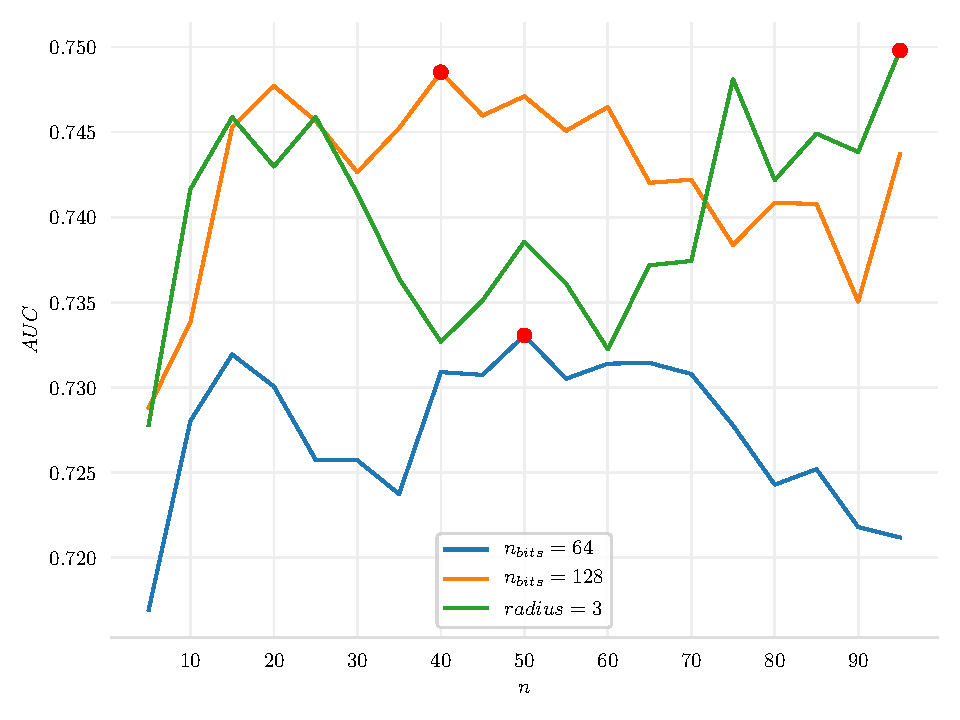
\includegraphics[width=\textwidth]{resources/pdf/knn-default-weight.pdf}
        \caption{Uniform weights}
    \end{subfigure}
    \begin{subfigure}{0.49\textwidth}
        \centering
        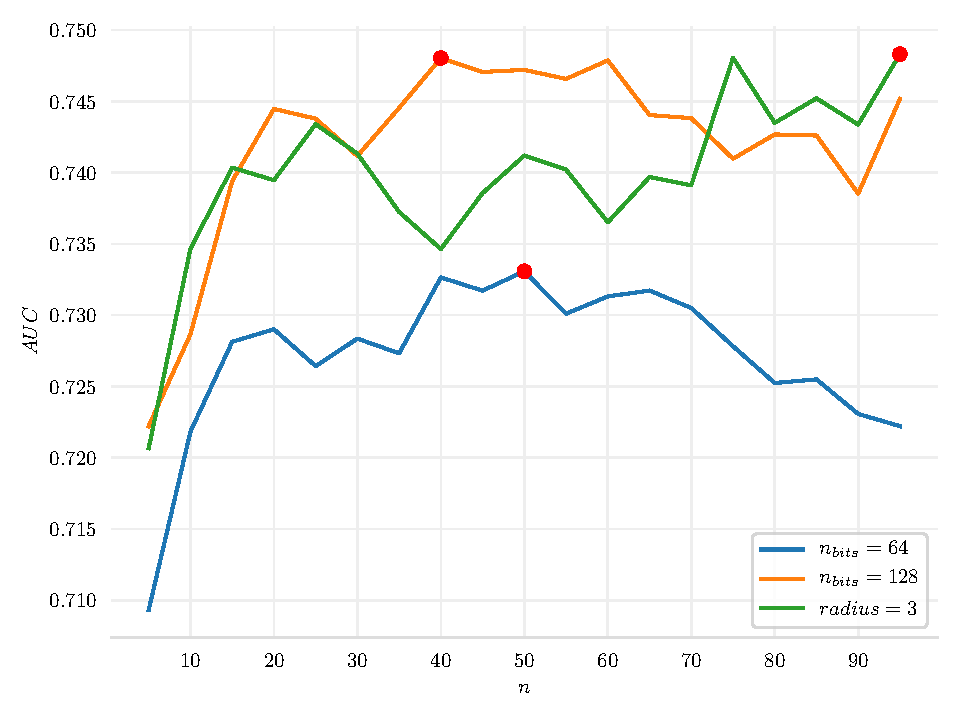
\includegraphics[width=\textwidth]{resources/pdf/knn-distance-weight.pdf}
        \caption{Anti-proportional weights}
    \end{subfigure}
    \caption{AUC estimation for KNN w.r.t. the numbers of neighbors.}
    \label{fig:knn_weight}
\end{figure}

\begin{figure}[h]
    \centering
    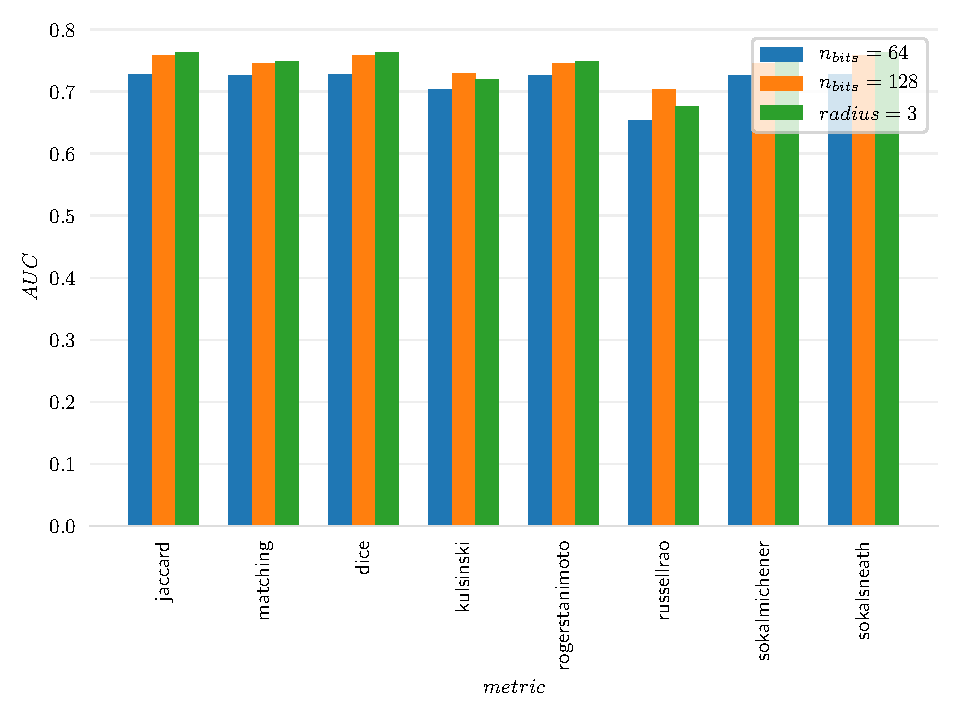
\includegraphics[width=0.59\textwidth]{resources/pdf/knn-metrics.pdf}
    \caption{AUC estimation for KNN w.r.t. the distance metric. (uniform weights and 20 neighbors)}
    \label{fig:knn_metrics}
\end{figure}

As one can see in Figures \ref{fig:knn_weight}, the uniform weights have the upper hand when fewer ($< 40$) neighbors are considered but it is the opposite afterwards, yet very slightly. By simplicity, we selected the uniform weights with $20$ neighbors which seemed a fine choice.

Concerning the metrics, it seems that none of them is significantly better than the default one. Once more by simplicity, we sticked to the default one.

What we can see, however, is that a greater number of bits induces better predictions. As stated above, this observation was made only at the end of the challenge, when we tried other fingerprints (increasing the number of bits with morgan did not provide better results for all models tested). If we had to provide another model, we would obviously increase \texttt{nBits} and use another fingerprint, as it would provide better results than the models we have designed.

\subsection{Multilayer perceptron}

The main elements of this method are the hidden layers shape and the activation function. We experienced a lot with the former and only a few with the latter. Indeed, changing the activation function for \texttt{'relu'} (default) to anything else seemed to worsen the results. We therefore varied the number of neurons per layer and the number of layers only.

\begin{figure}[h]
    \begin{subfigure}{0.49\textwidth}
        \centering
        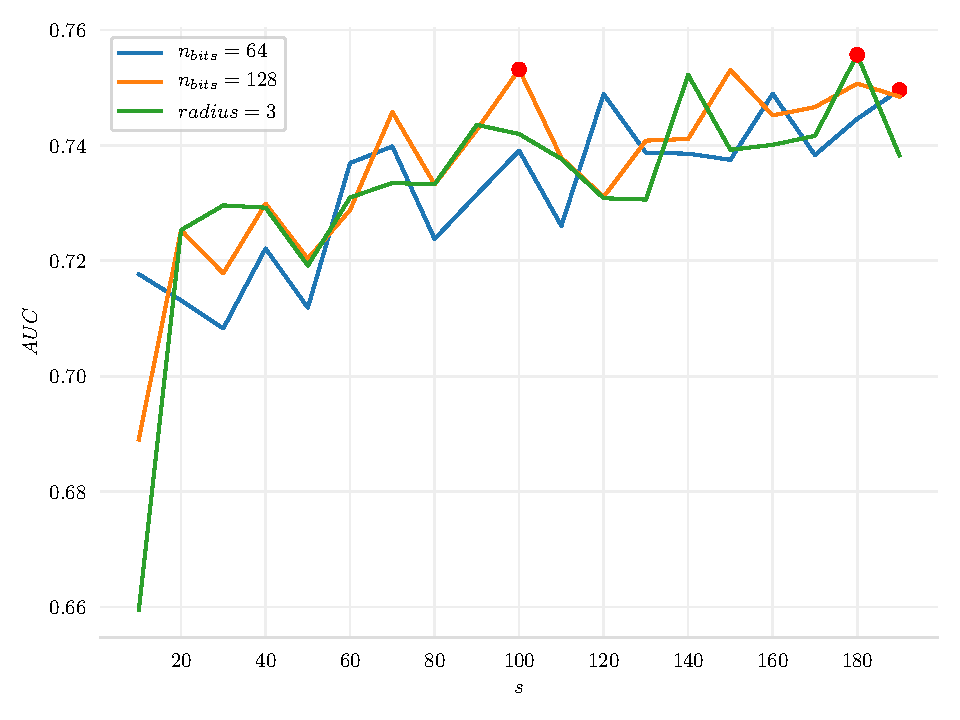
\includegraphics[width=\textwidth]{resources/pdf/mlp-layer-size.pdf}
        \caption{Number of neurons (1 layer)}
    \end{subfigure}
    \begin{subfigure}{0.49\textwidth}
        \centering
        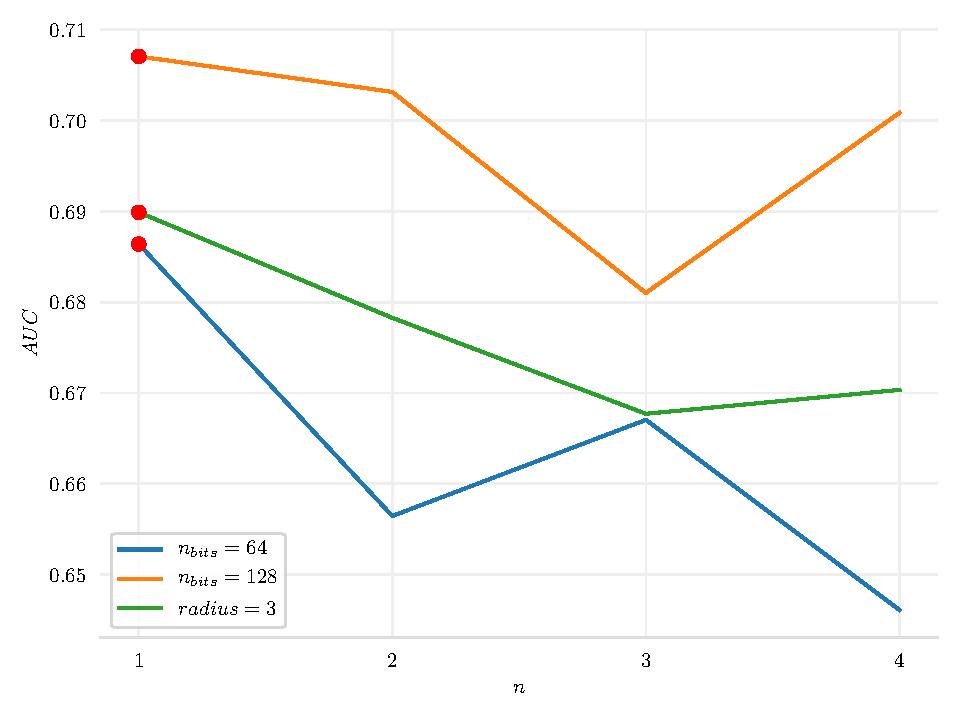
\includegraphics[width=\textwidth]{resources/pdf/mlp-layer-number.pdf}
        \caption{Number of layers (16 neurons per layer)}
    \end{subfigure}
    \caption{AUC estimation for MLP w.r.t. the shape of hidden layers.}
    \label{fig:mlp}
\end{figure}

Concerning the number of layers, it can be seen that the increase in the number of layers quickly degrades the score. A single layer seems to provide the best result. This is probably due to overfitting.

Concerning the number of neurons in the first layer, the score increases almost identically with all 3 Morgan fingerprints. A number of neurons between 100 and 200 seems to provide the best results.

\subsection{Random forest classifier}

The main parameter of this classifier is the number of trees in the forest. We therefore varied it while leaving the other parameters at their default values.

\begin{figure}[h]
    \begin{subfigure}{0.49\textwidth}
        \centering
        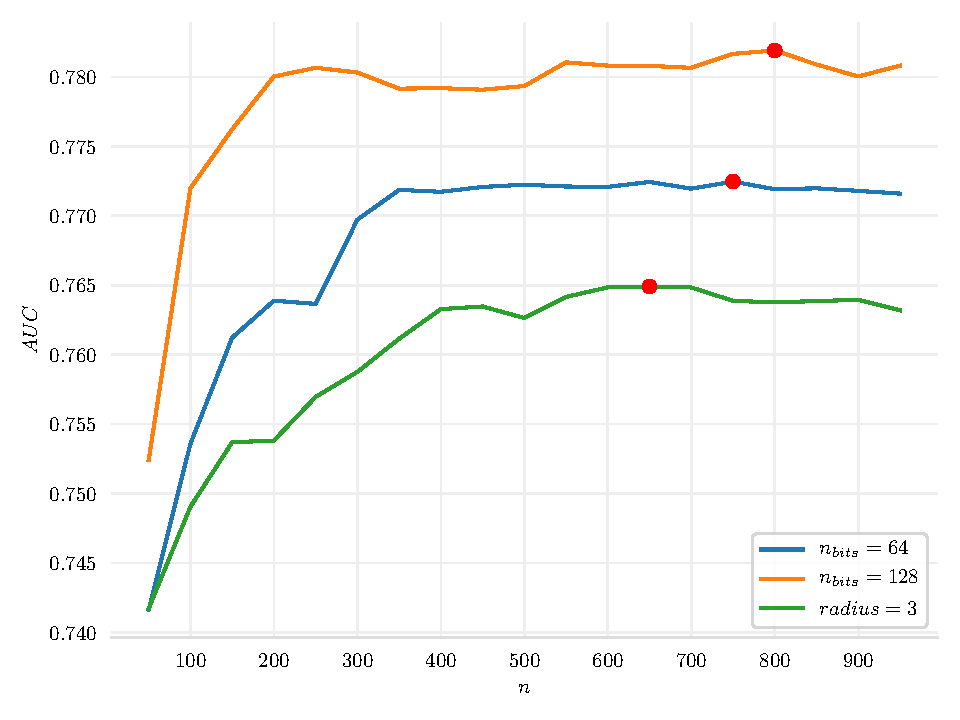
\includegraphics[width=\textwidth]{resources/pdf/rfc-number-trees.pdf}
        \caption{Unbalanced class weights}
    \end{subfigure}
    \begin{subfigure}{0.49\textwidth}
        \centering
        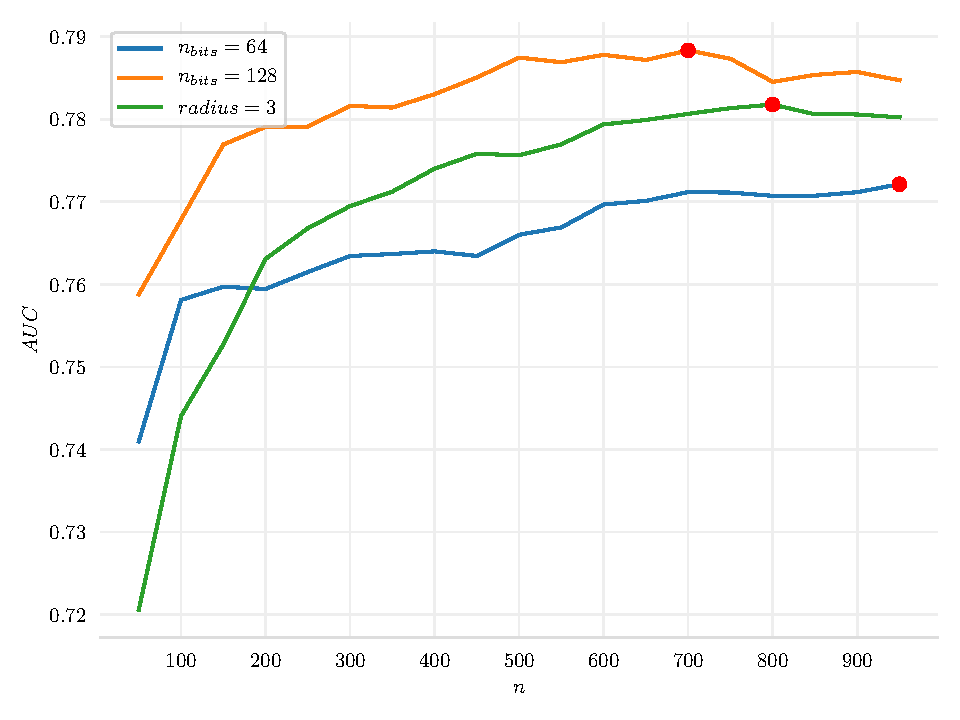
\includegraphics[width=\textwidth]{resources/pdf/rfc-number-trees-balanced.pdf}
        \caption{Balanced class weights}
    \end{subfigure}
    \caption{AUC estimation for RFC w.r.t. the number of trees.}
    \label{fig:rfc}
\end{figure}

In both cases (unbalanced and balanced class weights), the ROC AUC score appears to increase rapidly for a small number of trees and stabilizes when it increases.

In the unbalanced case, the score seems to stabilize at around 400 trees in the forest. There is a marked difference between the different parameters values for the Morgan fingerprint. The best result is, by far, obtained with 128 bits.

In the balanced case, the score stabilize later around 800 trees in the forest. The difference between fingerprint parameters is, in this case, less marked.

In both cases, the best score is obtain with Morgan using 128 bits. The score is slightly better in the balanced class weights case but the difference is very minimal.

\subsection{Support vector machine}

The main parameter of SVM is the kernel. Different kernels can deliver completely different predictions and each of them isn't suited to any problem. Therefore, we have implemented a few kernels inspired from the literature.

\begin{figure}[h]
    \centering
    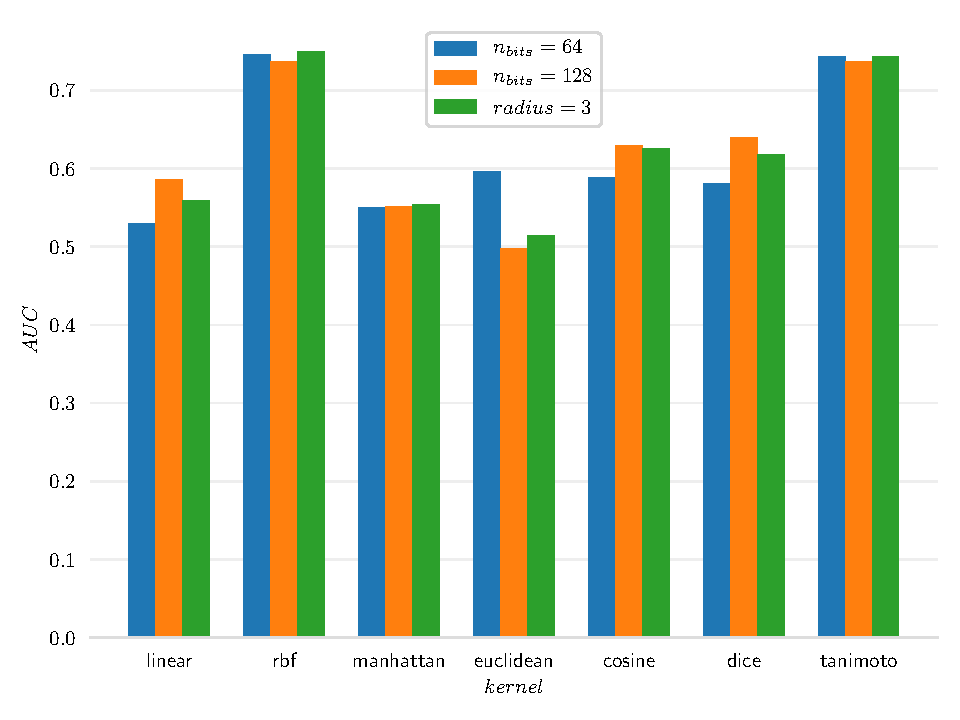
\includegraphics[width=0.66\textwidth]{resources/pdf/svm-kernels.pdf}
    \caption{AUC estimation for SVM w.r.t. the kernel.}
\end{figure}

As one can see, two kernels are largely above the others : the radial basis function (\texttt{rbf}) and the Tanimoto Similarity (\texttt{tanimoto}). Since \texttt{rbf} has one more tweaking parameter (\texttt{gamma}) than \texttt{tanimoto}, we chose it.

The other parameter of SVM is $C$, the regularization parameter. We can clearly see in the Figure \ref{fig:svm-c} that it has no influence on the predicted AUC.

\begin{figure}[h]
    \centering
    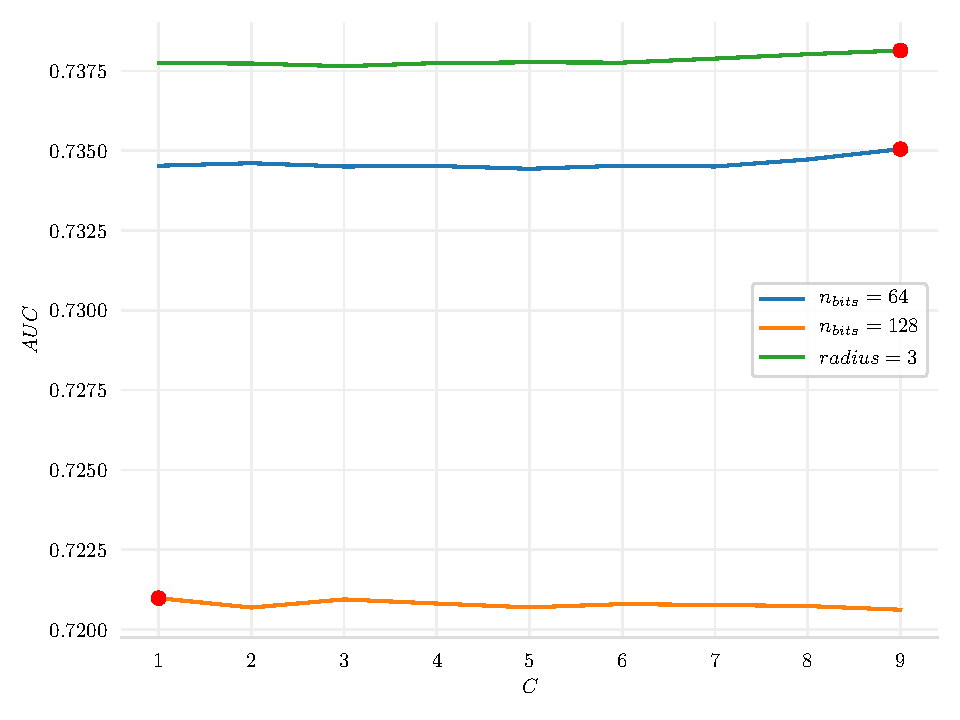
\includegraphics[width=0.66\textwidth]{resources/pdf/svm-c.pdf}
    \caption{AUC estimation for SVM w.r.t. $C$.}
    \label{fig:svm-c}
\end{figure}

\subsection{Ensemble models}

After testing some models individually in order to get an idea of their performance and the influence of their parameters on it, we tried to combine the best of them together.

The first way we tried was simply by averaging the probabilities of a set of chosen classifiers. This was done through the \texttt{VotingClassifier} of Scikit.

We also tried the \texttt{StackingClassifier} of mlxtend. This classifier doesn't average the probabilites, instead it trains another classifier (\texttt{meta\_classifier}) with the produced probabilities as input.

Finally, we designed our own ensemble classifier \texttt{ConsensusClassifier} which, as the two before, takes a list of unfitted classifiers as argument. However, instead of averaging the probabilities like the \texttt{VotingClassifier}, it computes the probability that a majority of classifier will vote \og{}in favour\fg{}.

Mathematically, we have a set $N$ of $n$ independent Bernoulli random variables $\mathcal{V}_i$ and their success probability $p_i$. Let $x$ be the number of successful variables $\mathcal{V}_i$. We have,
\begin{align*}
    P(x \geq j) & = \sum_{k = j}^{n} P(x = k) \\
    & = \sum_{k = j}^{n} \rbk{ \sum_{M \, \in \, C^k_N} P(\mathcal{V}_i = 1, \forall \, \mathcal{V}_i \in M) P(\mathcal{V}_i = 0,  \forall \, \mathcal{V}_i \in N \setminus M)} \\
    & = \sum_{k = j}^{n} \rbk{ \sum_{M \, \in \, C^k_N} \prod_{i \, \in \, M} p_i \prod_{i \, \in \, N \setminus M} (1 - p_i) }
\end{align*}
where $C^k_N$ represents the set of all $k$-combinations in $N$. Therefore, the probability computed by \texttt{ConsensusClassifier} is $$P\rbk{x \geq \frac{n + (n \bmod 2)}{2}} \, .$$

This model provides better results on our data than the two stated above, which is why this is the one we decided to keep for the tests and the final submission.

\subsection{Model Validation Technique}

In order to evaluate our models and decide if one was better than another, we decided to rely first on our prediction of the AUC. However, as these were not necessarily reflective of the score obtained on the public leaderboard, that score itself also played a role in our choices.

For example, for the submission \texttt{RFC(n\_estimators=500)} with \textit{MACCS} fingerprint (cf. Table \ref{tab:performance.summary}), we obtained an AUC estimation of \num{0.79} but a public score of \num{0.71}. We therefore decided to not investigate that fingerprint further, although the private score actually was \num{0.79} as well.

Retrospectively, we could have used other metrics to determine which model was better than another, and not base our decision only on the estimated AUC and the public score. As the public AUC was estimated from only one third of the test set, it could not be very reliable, as the classification problem was unbalanced.

The final models chosen are given at the end of the report.
